%----------------------------------------------------------
\chapter{Тестирование и отладка}\label{chap4_soft_testing}
%----------------------------------------------------------

\section{Экспорт графа в формате aDOT}
Рассмотрим работу редактора на примерах. Все примеры не имеют никакого математического смысла и приведены лишь для демонстрации работоспособности функционала редактора. Рассмотрим ориентированный граф созданный в редакторе с нуля, граф представлен на рисунке (\ref{fig:example_1}).

\begin{figure}[ht!]
\center{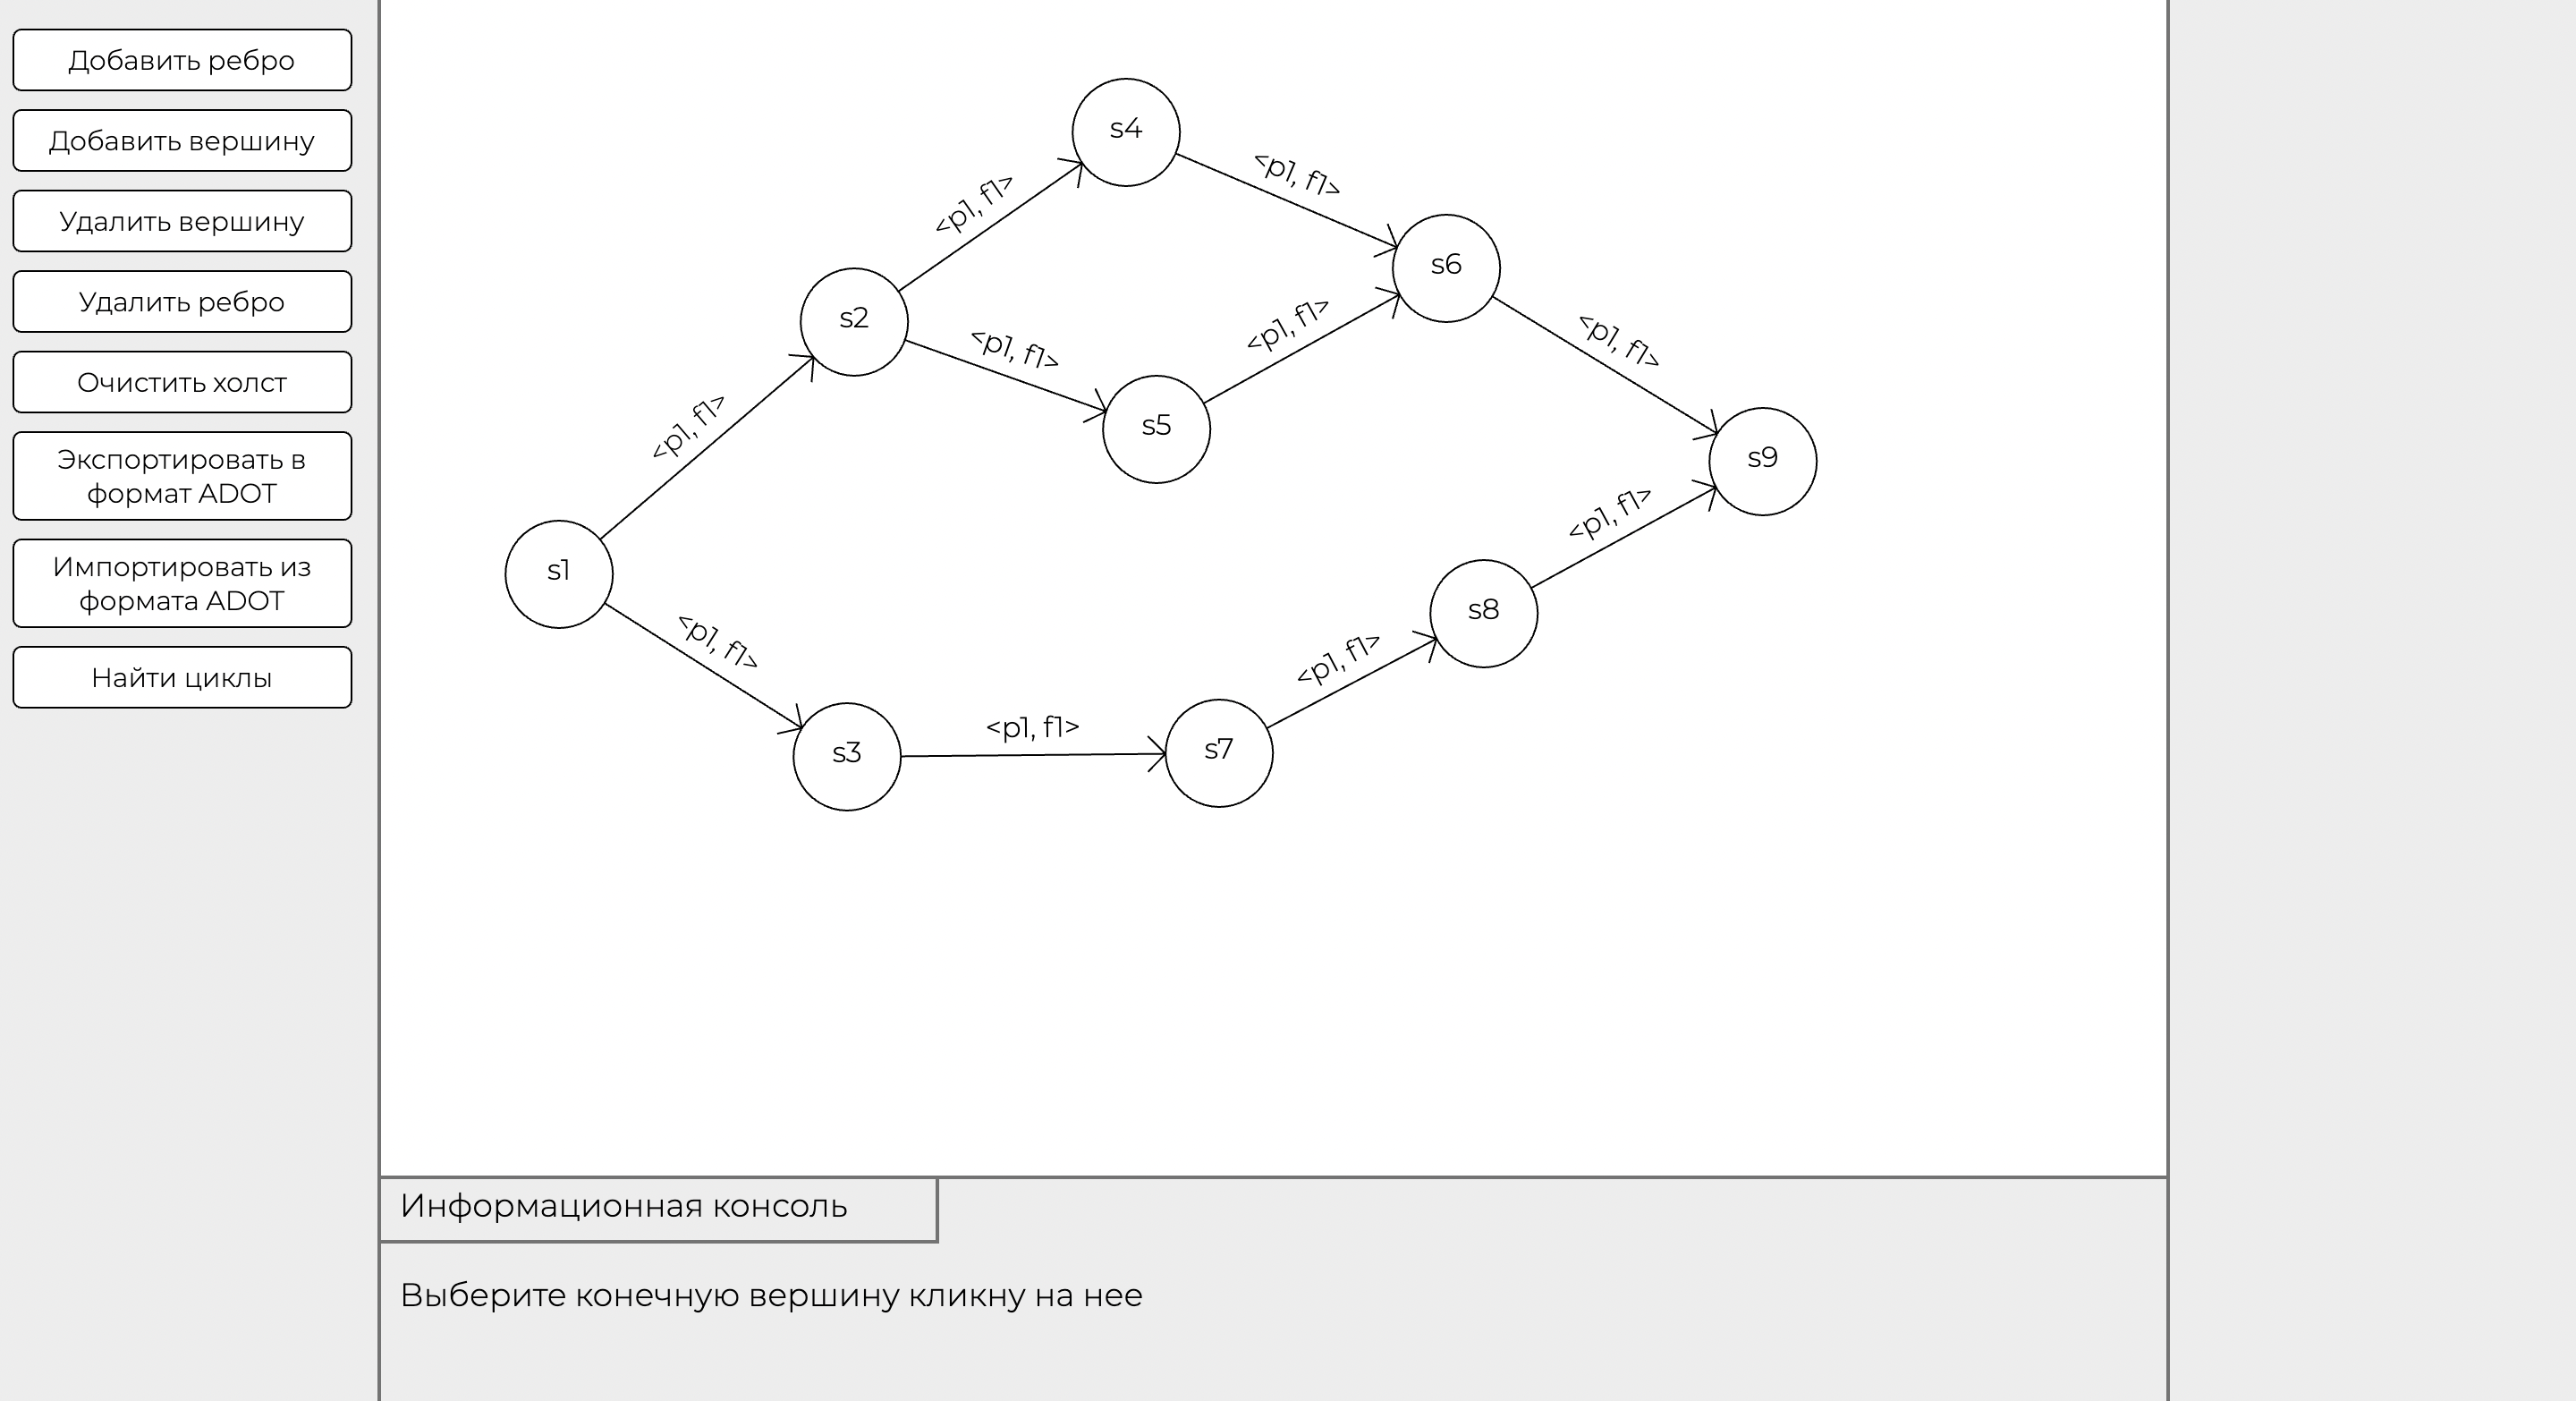
\includegraphics[width=0.9\linewidth]{images/example_1.png}}
\caption{Ориентированный граф созданный с нуля в редакторе}
\label{fig:example_1}
\end{figure}

Экспортируем построенный граф в формате aDOT. В результате будет получено следующее описание графовой модели в формате aDOT (листинг~\ref{lst:gm.exmpl.7}).

\begin{lstlisting}[label={lst:gm.exmpl.7}, caption={Полученное описание графовой модели (\ref{fig:example_1}) в формате aDOT}, language=JavaScript]
digraph TEST
{
// Parallelism
	s1 [parallelism=threading]
	s2 [parallelism=threading]
// Function
	f1 [module=f1_module, entry_func=f1_function]
// Predicates
	p1 [module=p1_module, entry_func=p1_function]
// Transition
	edge_1 [predicate=p1, function=f1]
// Graph model
	__BEGIN__ -> s1
	s1 => s2 [morphism=edge_1]
	s1 => s3 [morphism=edge_1]
	s2 => s4 [morphism=edge_1]
	s2 => s5 [morphism=edge_1]
	s3 -> s7 [morphism=edge_1]
	s4 -> s6 [morphism=edge_1]
	s5 -> s6 [morphism=edge_1]
	s6 -> s9 [morphism=edge_1]
	s7 -> s8 [morphism=edge_1]
	s8 -> s9 [morphism=edge_1]
	s9 -> __END__ 
}
\end{lstlisting}

Ранее было сказано, что задача экспорта графа является достаточно тривиальной, поэтому перейдем к рассмотрению примеров загрузки графа из формата aDOT.

\section{Импорт графа из формата aDOT}

В качестве первого примера рассмотрим описание графовой модели, которое было получено в предыдущем примере (листинг~\ref{lst:gm.exmpl.7}). После загрузки файла с описанием графовой модели получим граф представленный на рисунке (\ref{fig:example_1_imported}). Полученный граф выглядит более строго нежели этот же граф, но созданный вручную. Все вершины выровнены по оси Y относительно связанных с ними вершин.

\begin{figure}[ht!]
\center{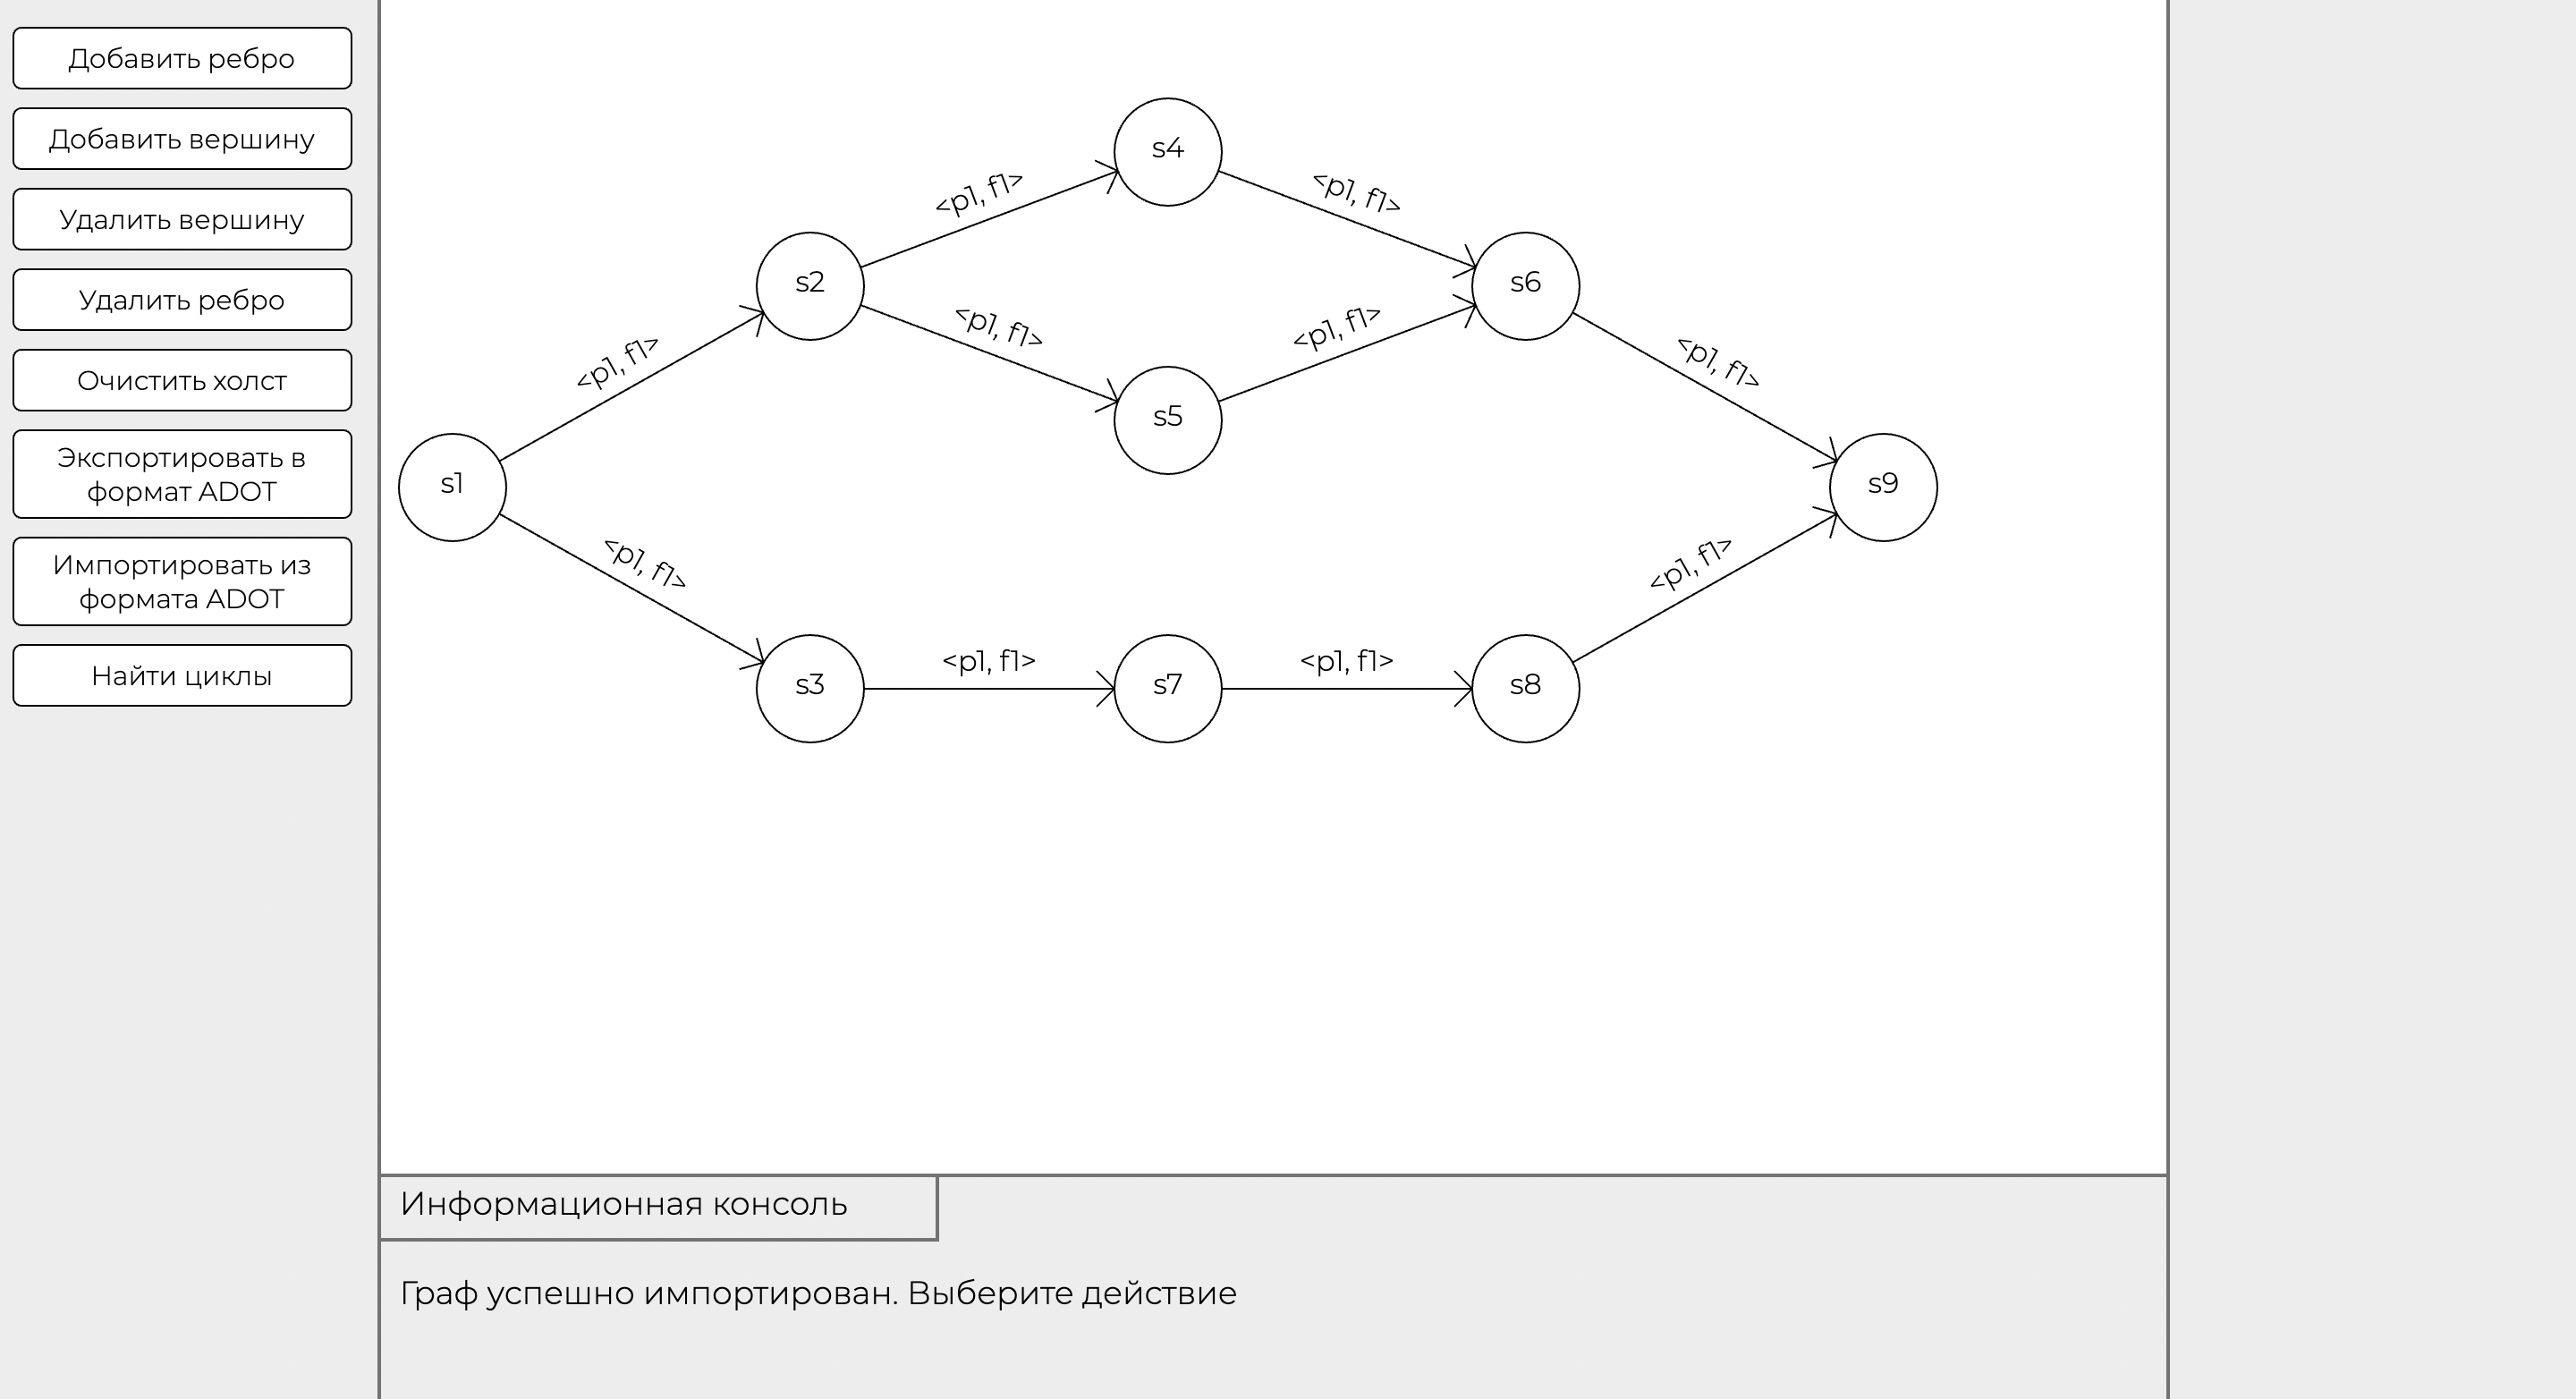
\includegraphics[width=0.8\linewidth]{images/example_1_imported.png}}
\caption{Загруженный в формате aDOT граф (листинг~\ref{lst:gm.exmpl.7})}
\label{fig:example_1_imported}
\end{figure}

Рассмотрим несколько других примеров, сначала будет представлено описание графовой модели в формате aDOT, а затем изображение полученного в результате графа.

\begin{lstlisting}[label={lst:gm.exmpl.8}, caption={Пример описание графовой модели в формате aDOT}, language=JavaScript]
digraph TEST
{
// Parallelism
	s2 [parallelism=threading]
	s1 [parallelism=threading]
	s10 [parallelism=threading]
// Function
	f1 [module=f1_module, entry_func=f1_function]
// Predicates
	p1 [module=p1_module, entry_func=p1_function]
// Transition
	edge_1 [predicate=p1, function=f1]
// Graph model
	__BEGIN__ -> s1
	s4 -> s6 [morphism=edge_1]
	s5 -> s6 [morphism=edge_1]
	s2 => s4 [morphism=edge_1]
	s2 => s5 [morphism=edge_1]
	s2 => s7 [morphism=edge_1]
	s1 => s2 [morphism=edge_1]
	s1 => s10 [morphism=edge_1]
	s6 -> s9 [morphism=edge_1]
	s8 -> s9 [morphism=edge_1]
	s7 -> s6 [morphism=edge_1]
	s10 => s11 [morphism=edge_1]
	s10 => s12 [morphism=edge_1]
	s11 -> s8 [morphism=edge_1]
	s12 -> s8 [morphism=edge_1]
	s9 -> __END__ 
}
\end{lstlisting}

\begin{figure}[ht!]
\center{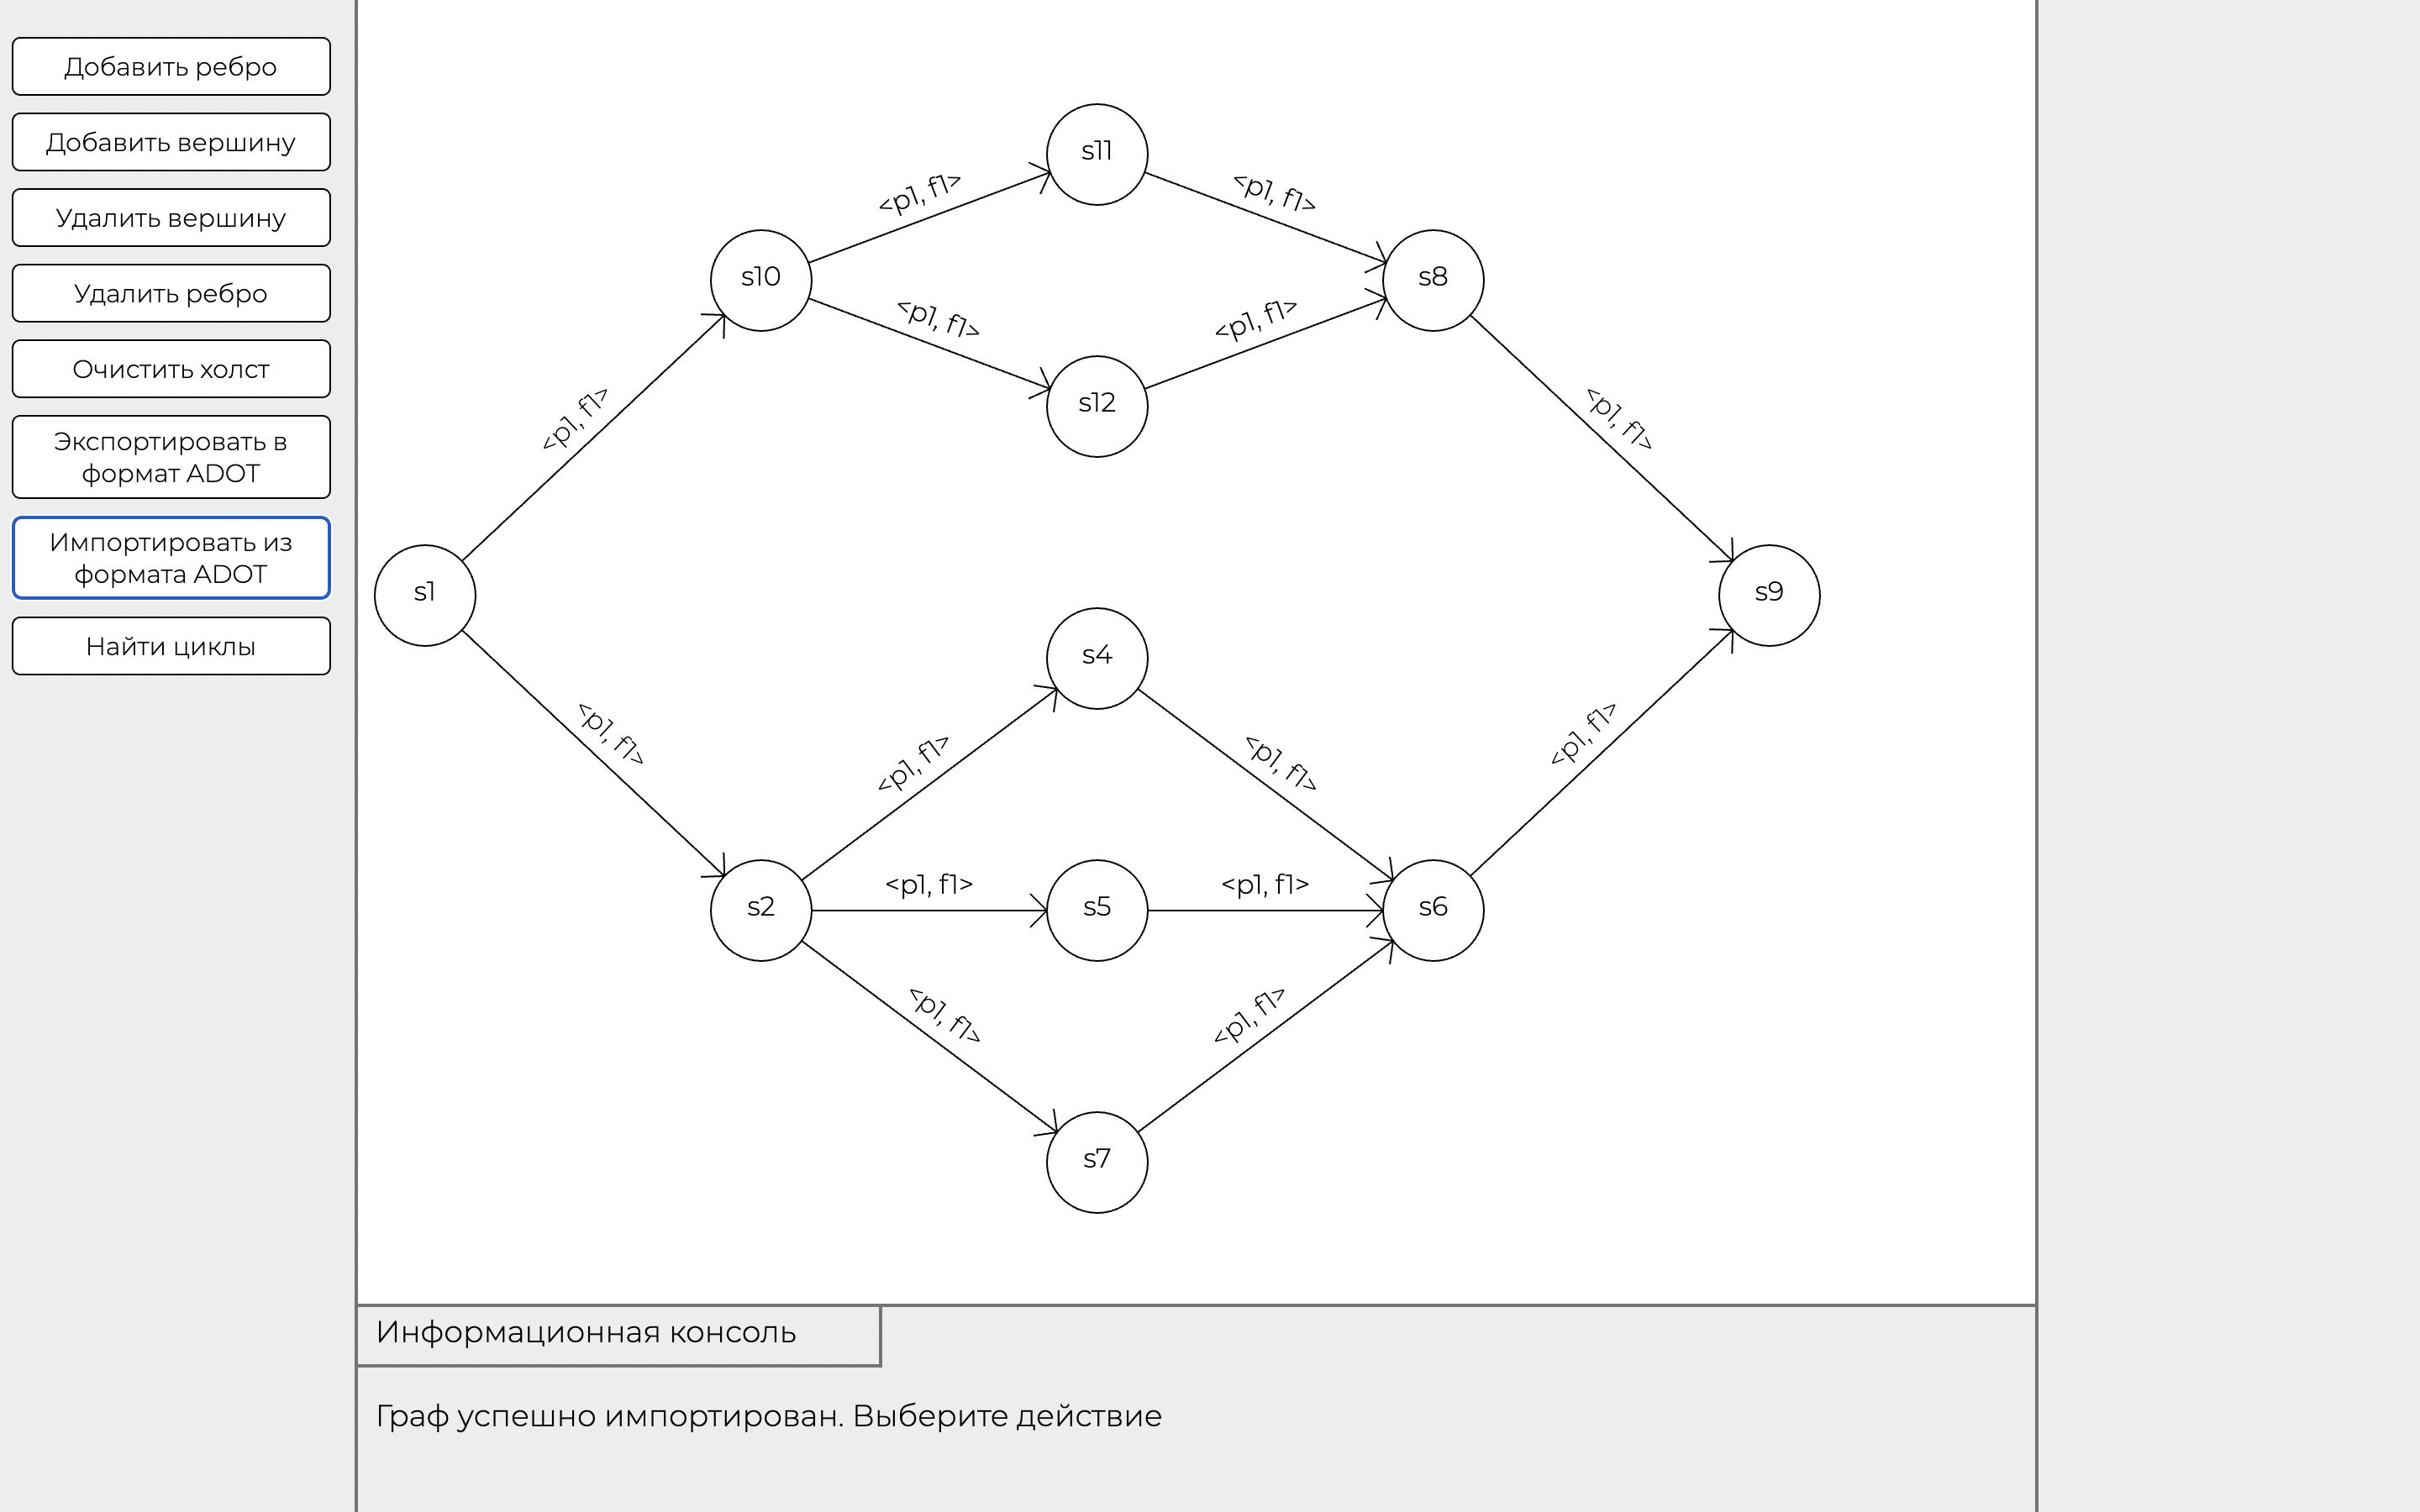
\includegraphics[width=0.8\linewidth]{images/example_2.png}}
\caption{Загруженный в формате aDOT граф (листинг~\ref{lst:gm.exmpl.8})}
\label{fig:example_2}
\end{figure}

В описание графовой модели (листинг~\ref{lst:gm.exmpl.8}) добавим несколько циклов и обратных ребер. Обратными ребрами будет называть ребра, которые выходят из вершины и приходят в вершину на уровне расположенном левее, при этом не формируя цикл. Получим следующее описание графовой модели 

\begin{lstlisting}[label={lst:gm.exmpl.9}, caption={Пример описание графовой модели в формате aDOT включающей циклы}, language=JavaScript]
digraph TEST
{
// Parallelism
	s7 [parallelism=threading]
	s11 [parallelism=threading]
	s2 [parallelism=threading]
	s10 [parallelism=threading]
	s1 [parallelism=threading]
// Function
	f1 [module=f1_module, entry_func=f1_function]
// Predicates
	p1 [module=p1_module, entry_func=p1_function]
// Transition
	edge_1 [predicate=p1, function=f1]
// Graph model
	__BEGIN__ -> s1
	s4 -> s6 [morphism=edge_1]
	s5 -> s6 [morphism=edge_1]
	s7 => s6 [morphism=edge_1]
	s7 => s1 [morphism=edge_1]
	s11 => s8 [morphism=edge_1]
	s11 => s2 [morphism=edge_1]
	s12 -> s8 [morphism=edge_1]
	s2 => s4 [morphism=edge_1]
	s2 => s5 [morphism=edge_1]
	s2 => s7 [morphism=edge_1]
	s10 => s11 [morphism=edge_1]
	s10 => s12 [morphism=edge_1]
	s1 => s2 [morphism=edge_1]
	s1 => s10 [morphism=edge_1]
	s6 -> s9 [morphism=edge_1]
	s8 -> s9 [morphism=edge_1]
	s9 -> s6 [morphism=edge_1]
	s9 -> __END__ 
}
\end{lstlisting}

~\\~\\


В таком случае будет построен граф представленный на рисунке (\ref{fig:example_3})

\begin{figure}[ht!]
\center{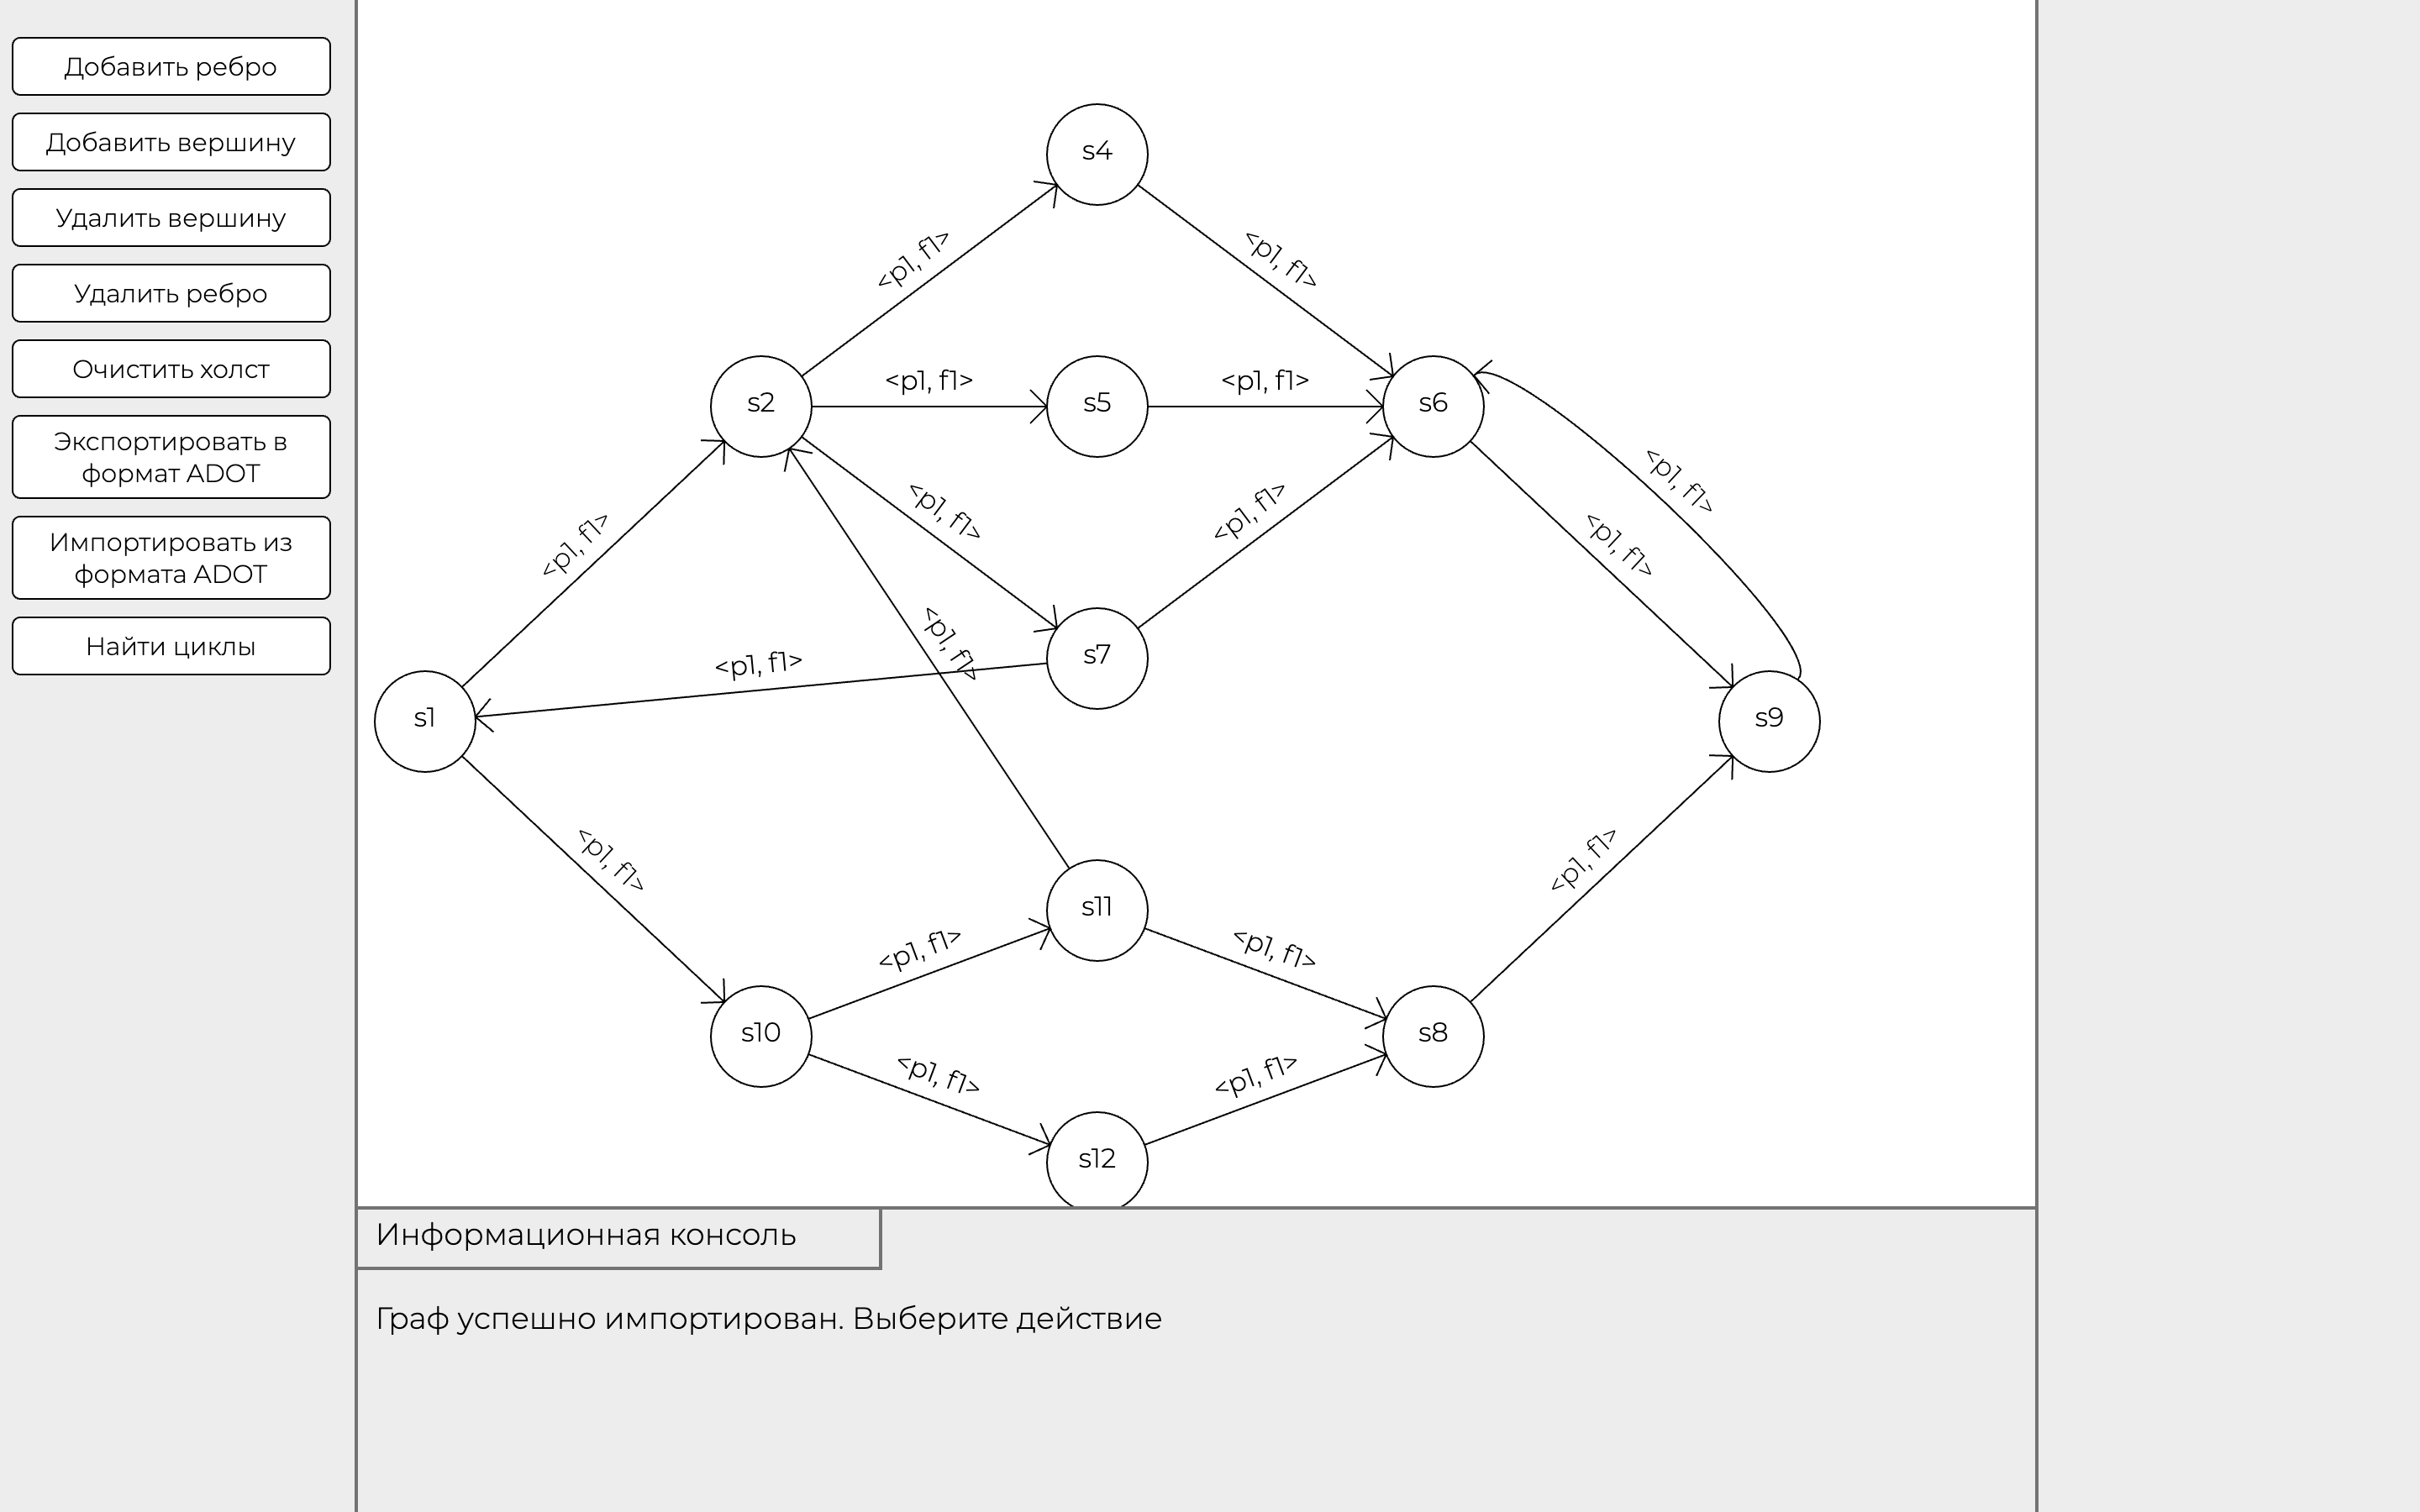
\includegraphics[width=0.8\linewidth]{images/example_3.png}}
\caption{Загруженный в формате aDOT граф (листинг~\ref{lst:gm.exmpl.9})}
\label{fig:example_3}
\end{figure}

Из примеров видно, что граф, который загружается из формата aDOT получается человекочитаемым. Расстояния между вершинами по оси X и по оси Y задаются через константы, что позволяет гибко настраивать размеры загружаемого графа - сделать его меньше или наоборот больше.



